\section{Experimental Results} 
\label{sec:results} 
 
In this section, we discuss the performance of several codes tuned with
Orio. We ran experiments on a multicore Intel Xeon machine and a Blue Gene/P
(both at Argonne National Laboratory). The Intel machine has dual quad-core
E5462 Xeon processors (eight cores in total) clocked at 2.8 GHz (1600 MHz
FSB) with 32 KB L1 cache, 12 MB of L2 cache (6 MB shared per core pair), and
2 GB of DDR2 FBDIMM RAM, running Linux kernel version 2.6.25 (x86-64). Each
compute node of the Blue Gene/P is equipped with four cores, each one a
850MHz IBM PowerPC 450 processors with a dual floating-point unit. While L1
cache (32 KB) and L2 cache (4 MB) are private for each processor, L3 cache (8
MB) is shared on each Blue Gene/P node. The total memory per node is 2GB. The
operating system on Blue Gene/P is based on Linux 2.6.16 (ppc64). ICC 10.1
and IBM XL C/C++ V9.0 were the primary compilers used on the Intel machine
and the Blue Gene/P, respectively.

\subsection{Sequence of Linear Algebra Operations} 
\label{sec:axpy4-results}
 
In this experiment, we tuned the performance of the AXPY-4 operation
(seen previously in Figure~\ref{fig:orio-example}) on a single node of
the Blue Gene/P machine using the IBM XLC compiler.  The performance
measurements were done for two cases: using a single core per node and using
all four cores, where the results can be found in
Figure~\ref{fig:axpy4-bgp-seq} and Figure~\ref{fig:axpy4-bgp-par},
respectively. The single-core scenario used the following compiler
options: \texttt{-O3 -qstrict -qarch=450d -qtune=450 -qhot
-qsmp=noauto}, whereas the multicore scenario differs in the use of
\texttt{-qsmp=auto} for the non-Orio versions. The parallel Orio
version contains OpenMP parallelization directives in generated code,
thus demanding the use of compiler option
\texttt{-qsmp=omp:noauto}. Included are performance numbers for four
code variants: a simple loop implementation with no any library calls
(labeled ``Compiler-optimized''), two BLAS-based implementations that
utilize the Goto BLAS~\cite{Goto:2006fk,Goto:fk} and the
ESSL~\cite{ESSL}, and the Orio-tuned version.

\begin{figure}[thb] 
\begin{center} 
  \subfigure[Sequential (single core)]{ 
  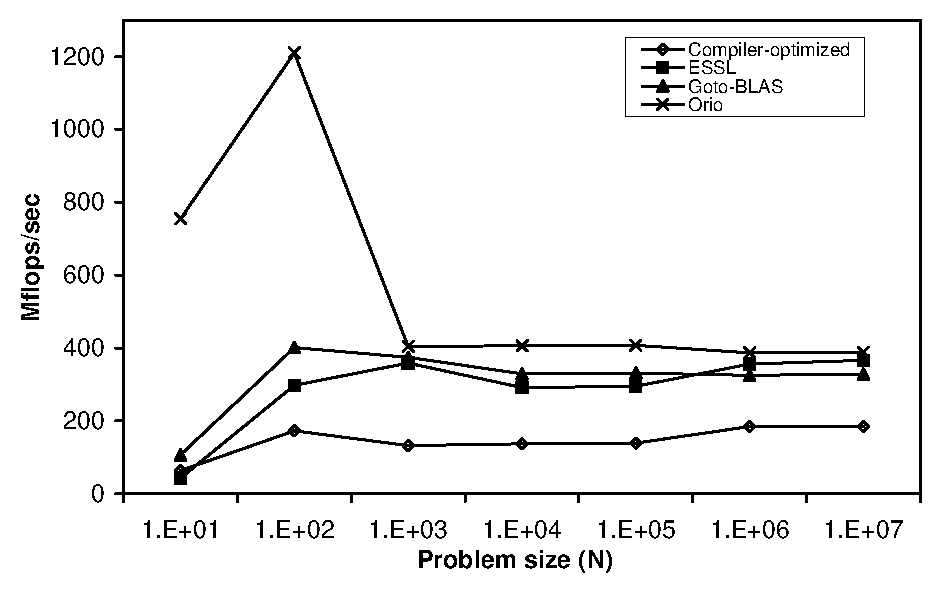
\includegraphics[width=.4\textwidth]{figures/axpy4_bgp/seq.eps}  
  \label{fig:axpy4-bgp-seq} 
  } 
  \subfigure[Parallel (four cores)]{ 
  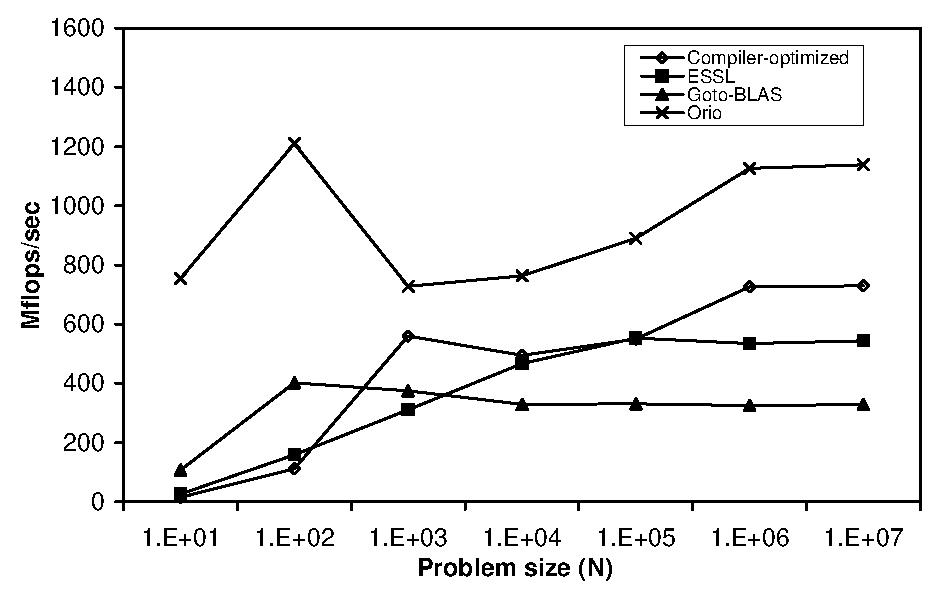
\includegraphics[width=.4\textwidth]{figures/axpy4_bgp/par.eps}  
  \label{fig:axpy4-bgp-par} 
  } 
\end{center}
\vspace{-.2in} 
\caption{Performance of AXPY-4 operations on Blue Gene/P} 
\label{fig:axpy4-bgp-results} 
\end{figure} 

The performance results shown in Figure~\ref{fig:axpy4-bgp-results}
indicate that the code version tuned by Orio consistently outperforms
all the other three versions for both the sequential and parallel
cases. It can be observed that even for a simple algebraic operation,
such as the composed AXPY routines, the compiler alone is unable to
yield performance comparable to the empirically tuned
version. Moreover, implementations that rely on calls to multiple
tuned library routines (e.g., Goto BLAS and ESSL) suffer from loss
both spatial and temporal localities, resulting in inferior memory
performance. The sequential performance results of the BLAS-based
implementations are higher than that of the single loop
implementation; while for the parallel case with high degree of
parallelism, the simple loop implementation is more efficient than the
BLAS codes.


\subsection{Sparse Matrix Computations} 

We examined the effectiveness of Orio in optimizing
PETSc~\cite{petsc-efficient}, a toolkit for the parallel numerical
solution of partial differential equations, by empirically tuning one
of its heavily used kernels: sparse matrix-vector multiplication
(SpMV). SpMV dominates the performance of various scientific
applications; yet, traditional implementations of sparse kernels are
relatively poor in performance. In order to attain higher performance,
SpMV requires selecting a compact data structure and code
transformations that best exploit properties of both the sparse matrix
and the underlying architecture. Hence, the need for optimization and
runtime tuning is a big distinction from the dense matrix-vector
multiplication.

SpMV operation takes in the form of $\forall_{A_{i,j}} \neq 0:y_{i}
\leftarrow y_{i} + A_{i,j} \cdot x_{j}$, where $A$ is a sparse matrix,
and $x$, $y$ are dense vectors. Each element of $A$ is used precisely
once and element reuse is only possible for $x$ and $y$. So,
optimizing SpMV should seek data structures for $A$ that are small and
maximize temporal reuse of $x$ and $y$. The most widespread data
structure used for storing a sparse matrix is compressed sparse row
(CSR)~\cite{vuduc-thesis} storage, as shown in
Figure~\ref{fig:spmv}(a). Elements in each row of $A$ are packed
together in a dense array, \texttt{Aval}, and a corresponding array of
integers \texttt{Aind} stores the column indices. The \texttt{Aptr}
array designates where each sparse row begins in \texttt{Aval} and
\texttt{Aind}. A direct implementation of SpMV using CSR storage is
presented in Figure~\ref{fig:spmv}(b).

\begin{figure}[htp]
\centering
\vspace{.2in}
\begin{tabular}{cc}
\begin{minipage}[b]{.5\textwidth}
\centering
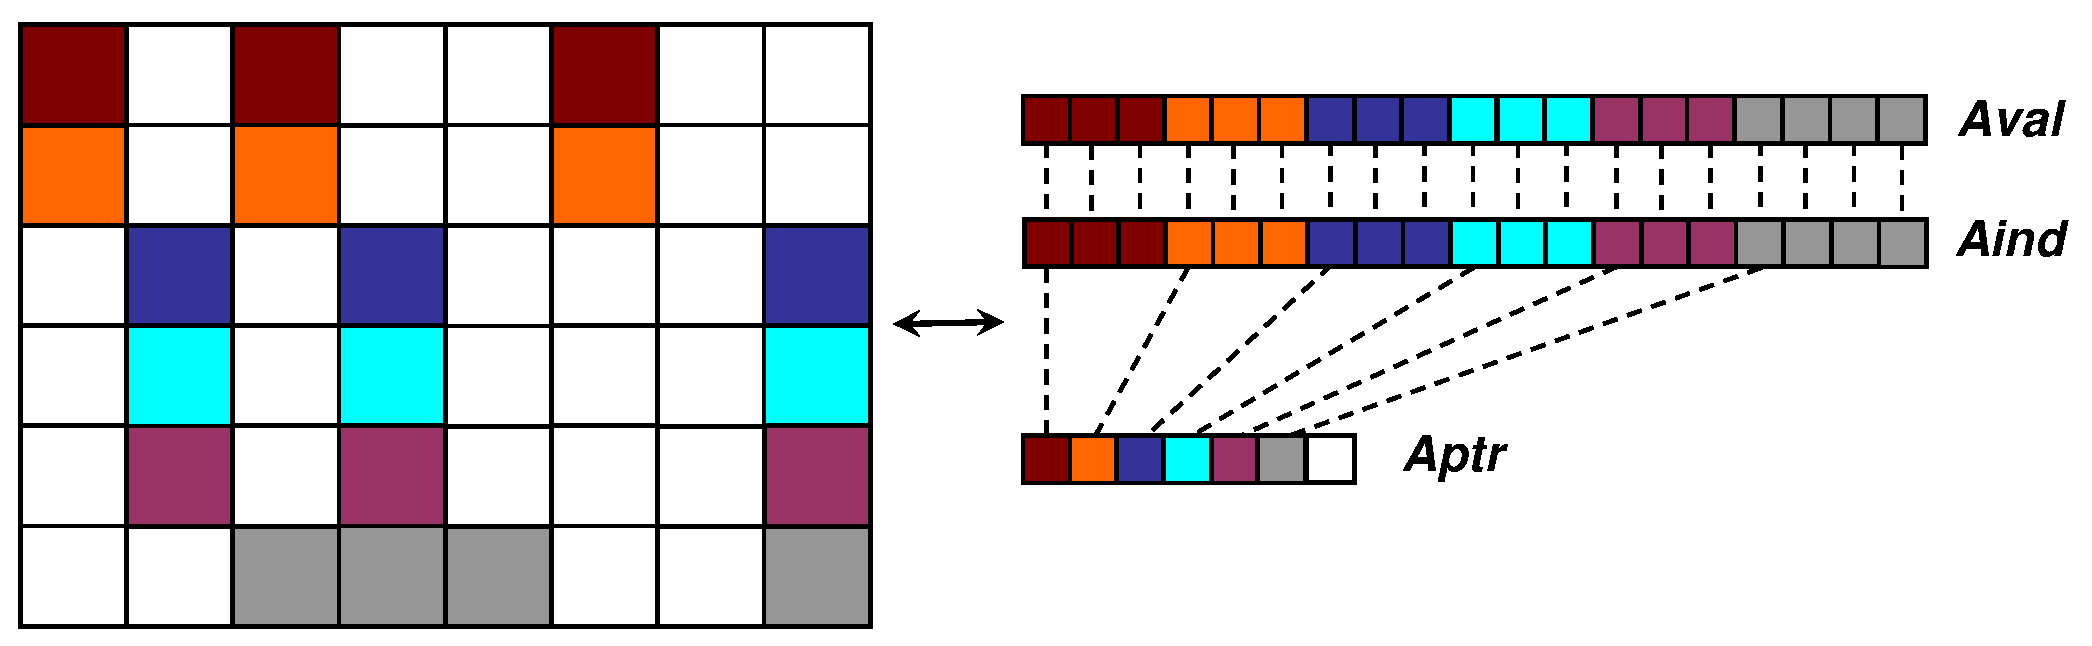
\includegraphics[width=.8\textwidth]{figures/spmv.eps}  
\end{minipage}
&
\begin{minipage}[b]{.5\textwidth}
\scriptsize
\begin{verbatim}
for (i=0; i<num_rows; i++)
  for (j=Aptr[i]; j<Aptr[i+1]; j++)
    y[i] += Aval[j]*x[Aind[j]];


\end{verbatim}
\end{minipage}\\
(a) & (b)\\
\end{tabular}
\vspace{-.1in}
\caption{(a) Compressed sparse row (CSR) format (b) Basic implementation of CSR-based SpMV}
\label{fig:spmv}
\end{figure}

The PETSc's SpMV used in this experiment exploits \textit{inode}
format, which takes advantage of rows with identical nonzero
structure. For example, the sparse matrix portrayed in
Figure~\ref{fig:spmv}(a) consists of three inodes. The first inode has
the size of two as it holds two adjacent rows (i.e., the first and the
second rows) with the same nonzero structure. The second inode
contains three consecutive rows with identical nonzero structure,
while the last inode only has a single row. Knowing the properties of
each inode at runtime enables maximum reuse of vector $x$ since
multiple elements of $x$ can be loaded and used exactly once for all
rows in the same inode structure. To do this requires the usage of
register-blocking transformation. In order to optimize inode-based
SpMV routine, we incorporated a new transformation module inside Orio
that implements various optimization strategies including register
blocking, SIMDization, memory alignment optimization, loop-control
optimization, accumulator expansion, and thread-level parallelization
(with OpenMP). We then used Orio to automatically select the best
version of the optimized inode SpMV. It is noted that the loop to be
parallelized with OpenMP is the outer most loop that iterates over
each inode structure.


\begin{figure} [thb]
\begin{center} 
  \subfigure[1 node, SMP mode]{ 
  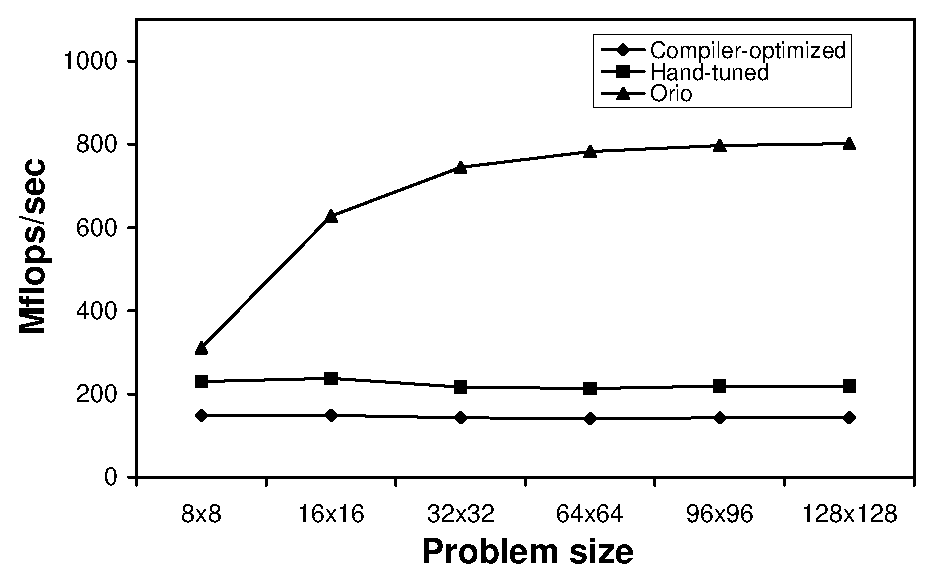
\includegraphics[width=.3\textwidth]{figures/ex27_bgp/n1_smp.eps}  
  \label{fig:ex27-bgp-smp-n1} 
  } 
  \subfigure[1 node, Dual mode]{ 
  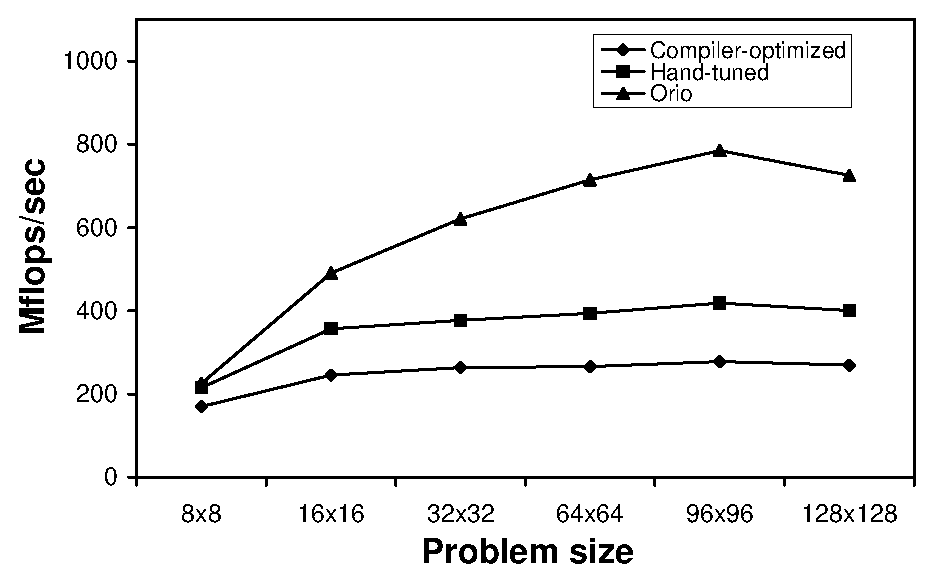
\includegraphics[width=.3\textwidth]{figures/ex27_bgp/n1_dual.eps}  
  \label{fig:ex27-bgp-dual-n1} 
  } 
  \subfigure[1 node, VN mode]{ 
  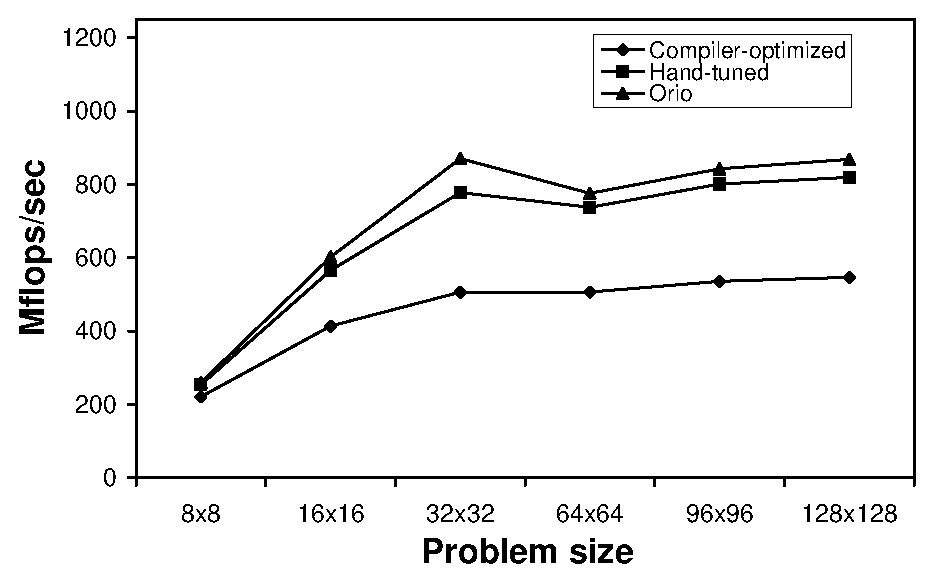
\includegraphics[width=.3\textwidth]{figures/ex27_bgp/n1_vn.eps}  
  \label{fig:ex27-bgp-vn-n1} 
  } 
  \subfigure[8 nodes, SMP mode]{ 
  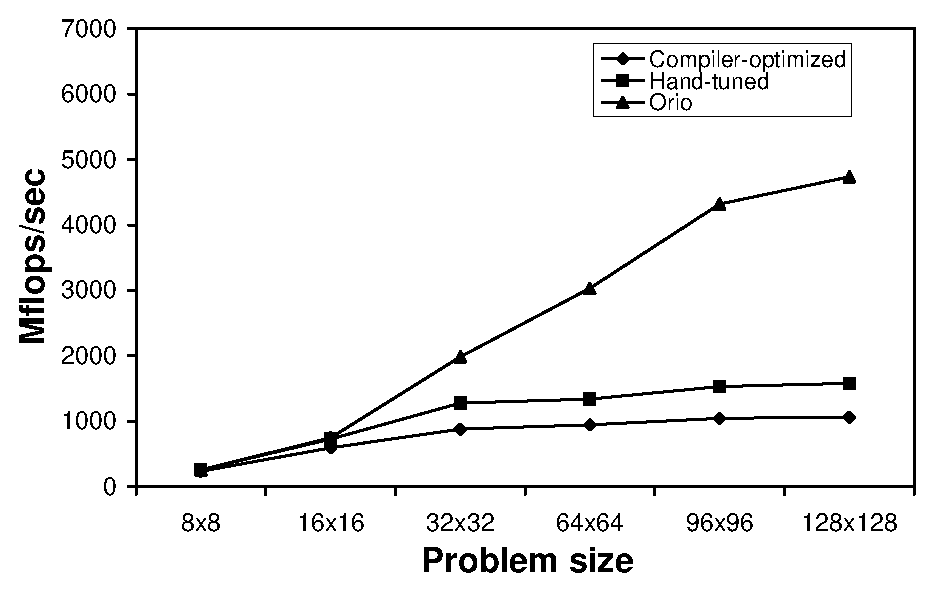
\includegraphics[width=.3\textwidth]{figures/ex27_bgp/n8_smp.eps}  
  \label{fig:ex27-bgp-smp-n8} 
  } 
  \subfigure[8 nodes, Dual mode]{ 
  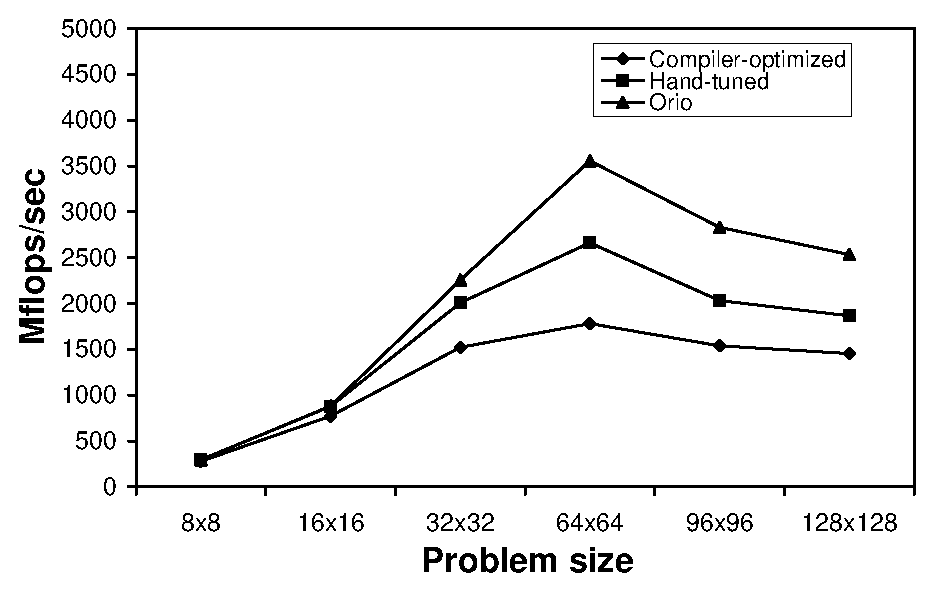
\includegraphics[width=.3\textwidth]{figures/ex27_bgp/n8_dual.eps}  
  \label{fig:ex27-bgp-dual-n8} 
  } 
  \subfigure[8 nodes, VN mode]{ 
  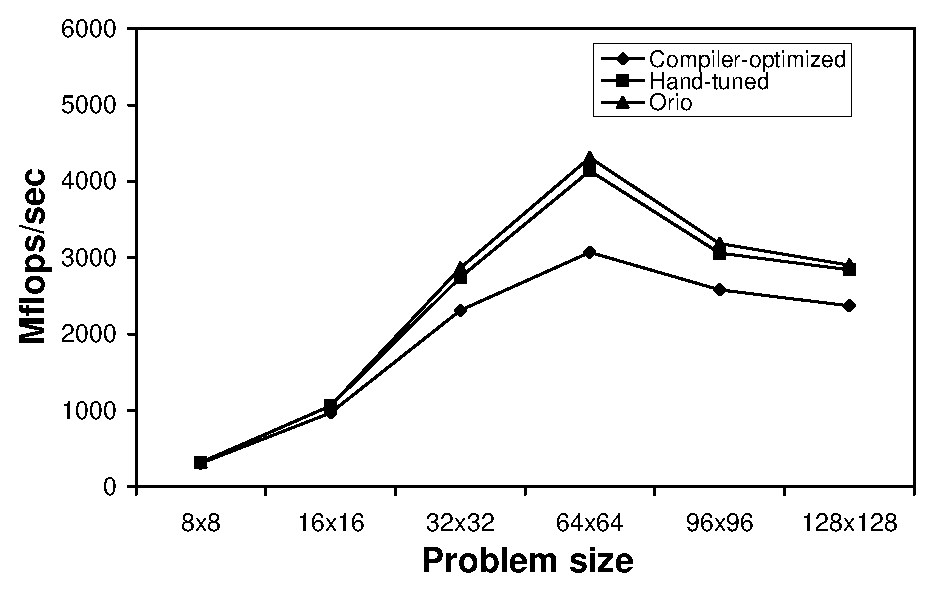
\includegraphics[width=.3\textwidth]{figures/ex27_bgp/n8_vn.eps}  
  \label{fig:ex27-bgp-vn-n8} 
  } 
  \subfigure[32 nodes, SMP mode]{ 
  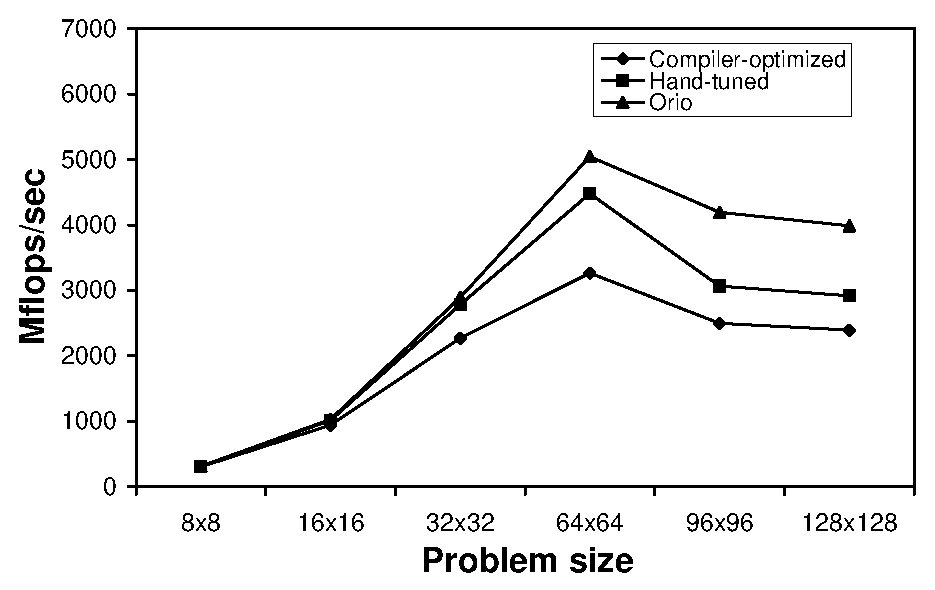
\includegraphics[width=.3\textwidth]{figures/ex27_bgp/n32_smp.eps}  
  \label{fig:ex27-bgp-smp-n32} 
  } 
  \subfigure[32 nodes, Dual mode]{ 
  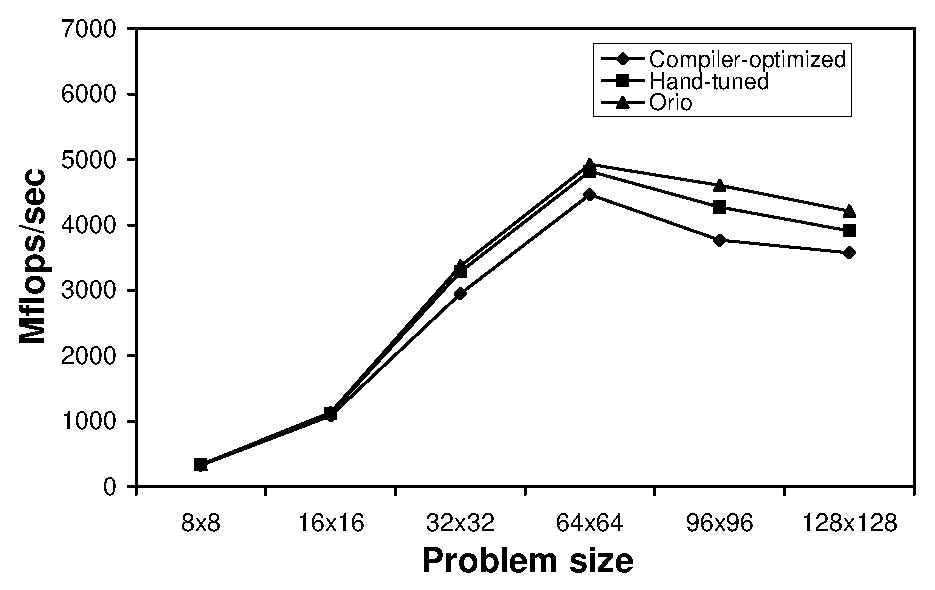
\includegraphics[width=.3\textwidth]{figures/ex27_bgp/n32_dual.eps}  
  \label{fig:ex27-bgp-dual-n32} 
  } 
  \subfigure[32 nodes, VN mode]{ 
  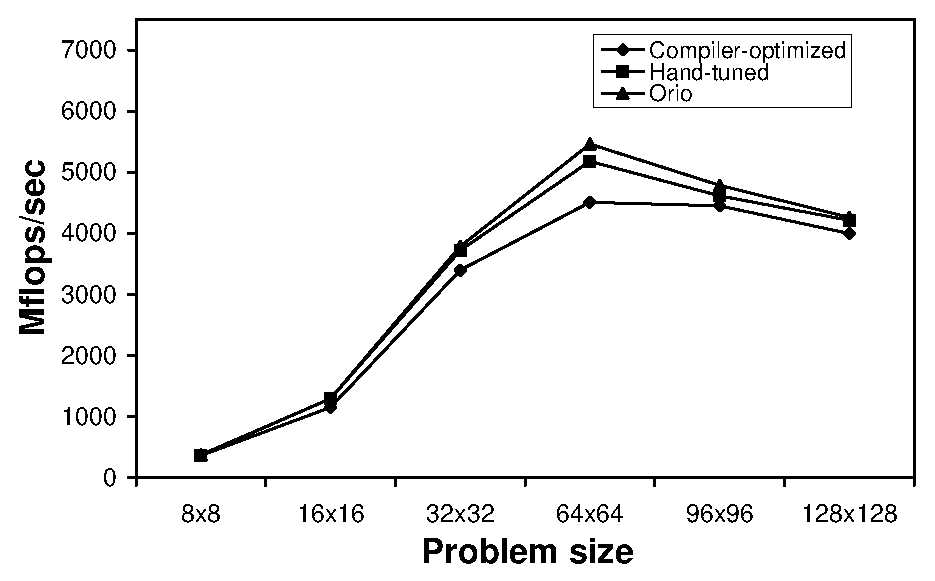
\includegraphics[width=.3\textwidth]{figures/ex27_bgp/n32_vn.eps}  
  \label{fig:ex27-bgp-vn-n32} 
  } 
\end{center}
\vspace{-.2in} 
\caption{Performance of inode SpMV on Blue Gene/P for 1, 8, and 32 nodes.} 
\label{fig:ex27-bgp-results1} 
\end{figure} 

\comment{
\begin{figure} 
\begin{center} 
  \subfigure[32x32, SMP mode]{ 
  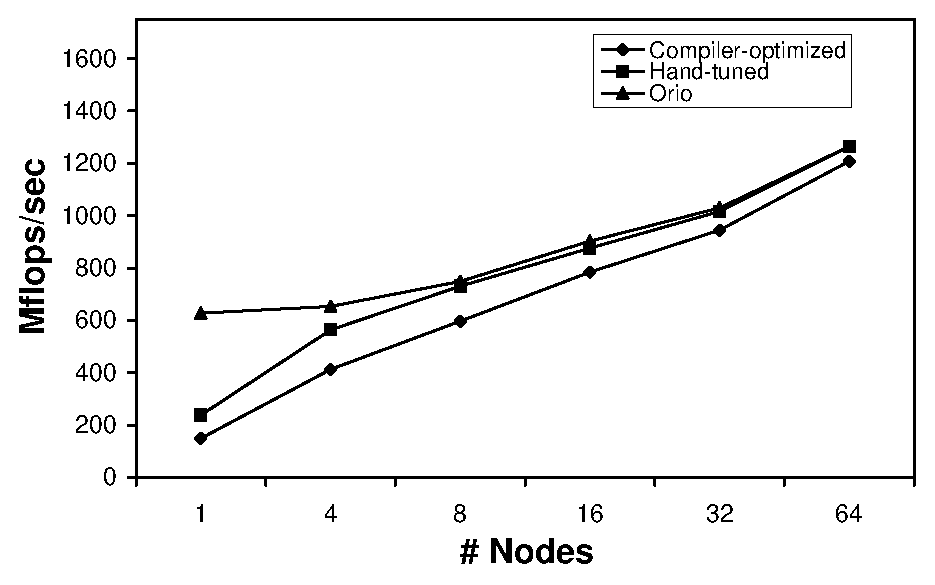
\includegraphics[width=.3\textwidth]{figures/ex27_bgp/s32_smp.eps}  
  \label{fig:ex27-bgp-smp-32x32} 
  } 
  \subfigure[32x32, Dual mode]{ 
  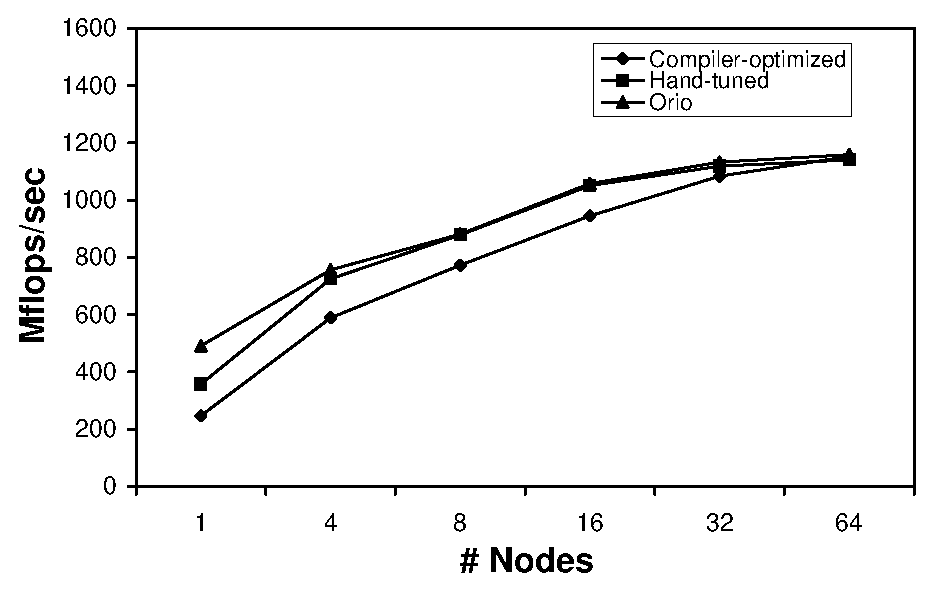
\includegraphics[width=.3\textwidth]{figures/ex27_bgp/s32_dual.eps}  
  \label{fig:ex27-bgp-dual-32x32} 
  } 
  \subfigure[32x32, VN mode]{ 
  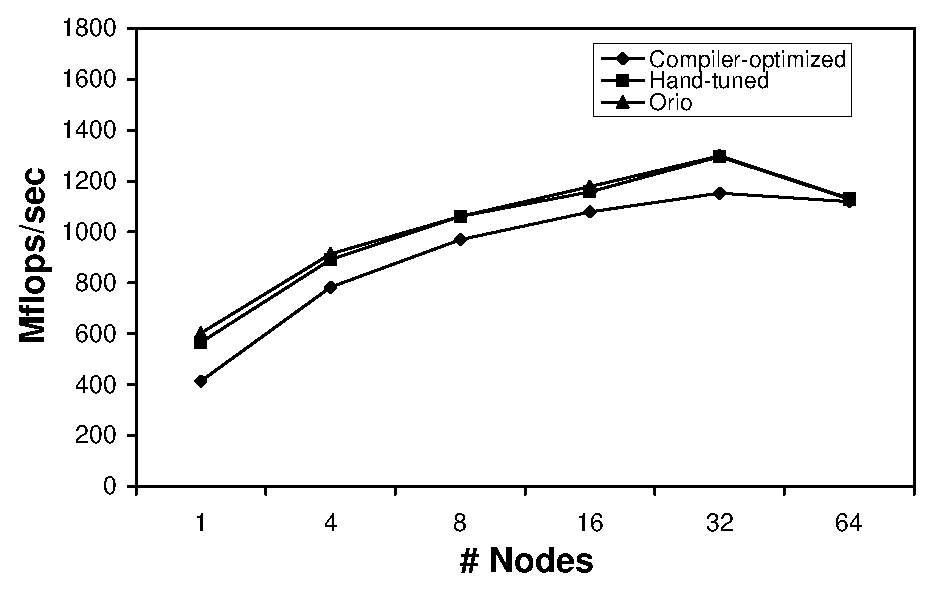
\includegraphics[width=.3\textwidth]{figures/ex27_bgp/s32_vn.eps}  
  \label{fig:ex27-bgp-vn-32x32} 
  } 
  \subfigure[64x64, SMP mode]{ 
  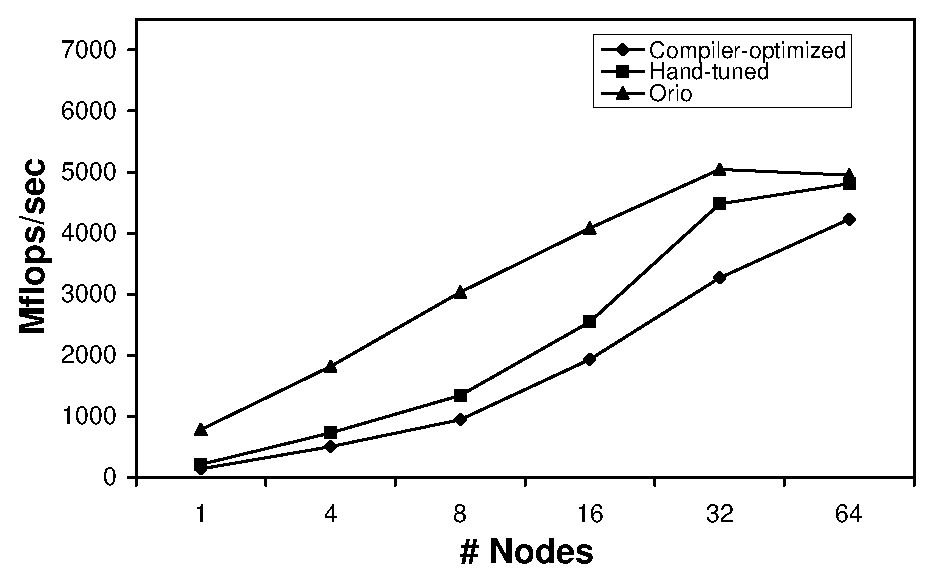
\includegraphics[width=.3\textwidth]{figures/ex27_bgp/s64_smp.eps}  
  \label{fig:ex27-bgp-smp-64x64} 
  } 
  \subfigure[64x64, Dual mode]{ 
  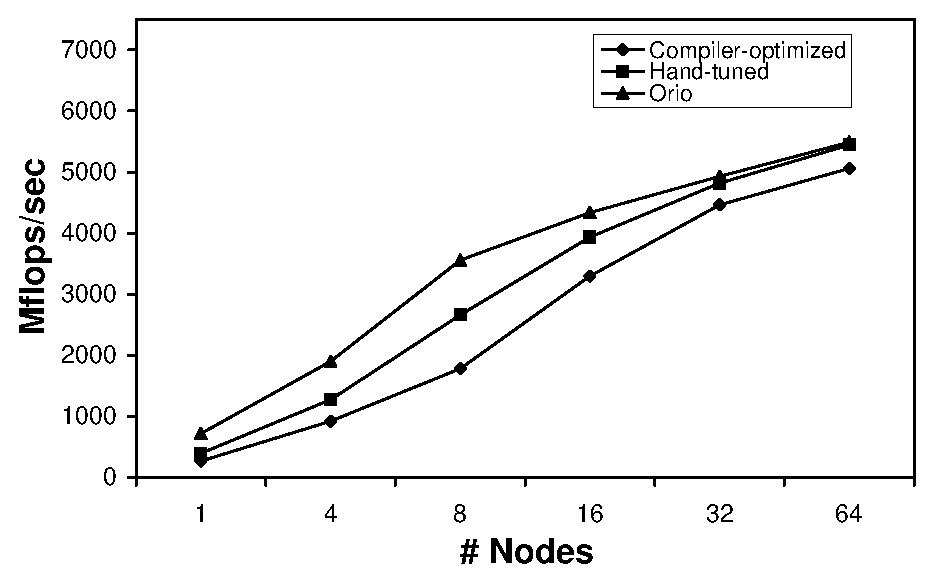
\includegraphics[width=.4\textwidth]{figures/ex27_bgp/s64_dual.eps}  
  \label{fig:ex27-bgp-dual-64x64} 
  } 
  \subfigure[64x64, VN mode]{ 
  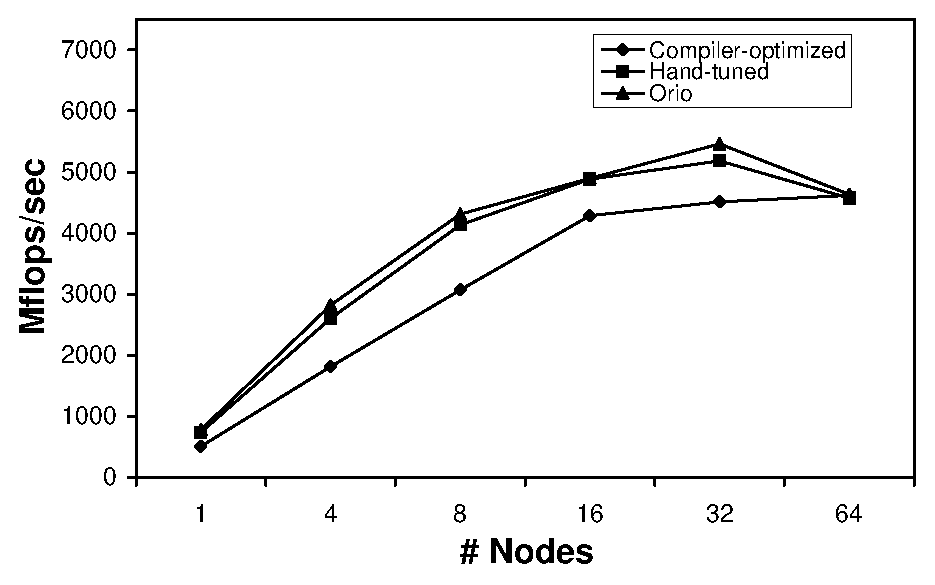
\includegraphics[width=.3\textwidth]{figures/ex27_bgp/s64_vn.eps}  
  \label{fig:ex27-bgp-vn-64x64} 
  } 
  \subfigure[128x128, SMP mode]{ 
  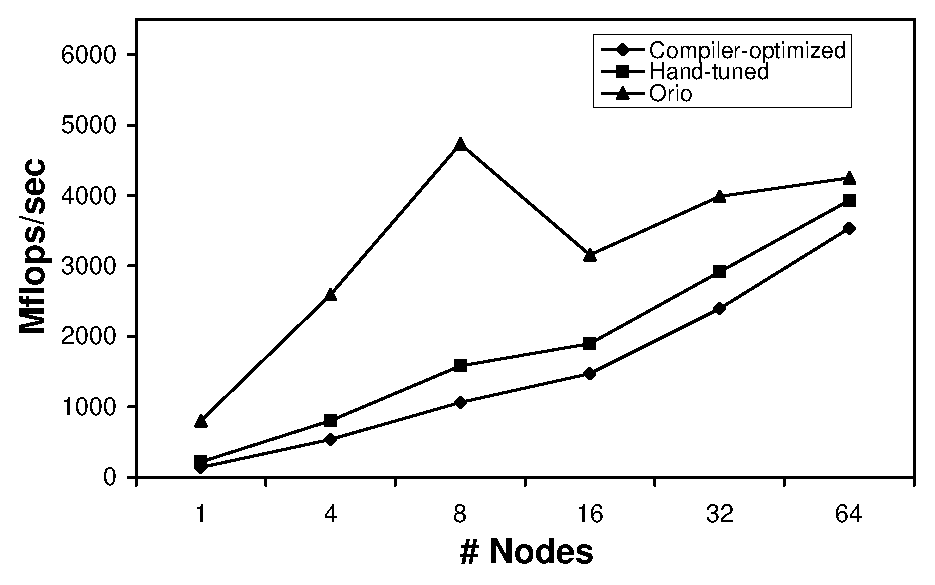
\includegraphics[width=.3\textwidth]{figures/ex27_bgp/s128_smp.eps}  
  \label{fig:ex27-bgp-smp-128x128} 
  } 
  \subfigure[128x128, Dual mode]{ 
  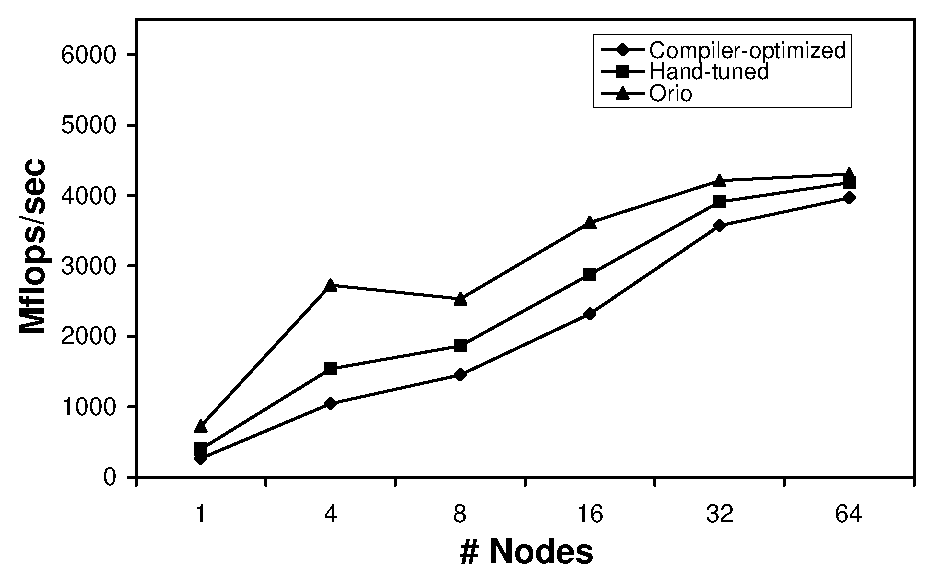
\includegraphics[width=.3\textwidth]{figures/ex27_bgp/s128_dual.eps}  
  \label{fig:ex27-bgp-dual-128x128} 
  } 
  \subfigure[128x128, VN mode]{ 
  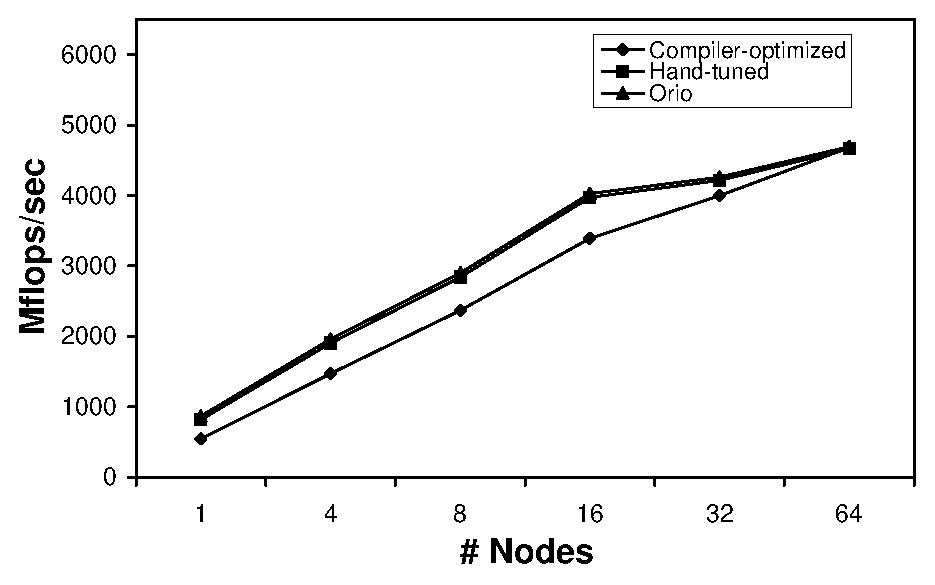
\includegraphics[width=.3\textwidth]{figures/ex27_bgp/s128_vn.eps}  
  \label{fig:ex27-bgp-vn-128x128} 
  } 
\end{center}
\vspace{-.2in}
\caption{Performance of inode SpMV on Blue Gene/P for problem sizes 32x32, 64x64, and 128x128.} 
\label{fig:ex27-bgp-results2} 
\end{figure} 
}

To evaluate the performance of the tuned SpMV routine, we conduct the
experiment using one of actual application simulations of PETSc,
called \textit{Nonlinear 2-D Driven Cavity} problem, on both the
multicore Intel machine and Blue Gene/P. The ``Compiler-optimized''
label is used as a base comparison that represents the performance of
the naive implementation of SpMV (shown in Figure~\ref{fig:spmv}(b))
optimized by the native compiler. We also tested the performance of
the hand-tuned SpMV code that is already integrated in the PETSc
releases.

Figure~\ref{fig:ex27-cookie-results} exhibits the performance speedups
accomplished by Orio on the Intel Xeon machine. To be noted that the
input problem size signifies the number of grid points in $x$ and $y$
directions, not the size of the sparse input matrix. In this
experiment, we utilized all available cores by running PETSc in three
different modes: SMP (one MPI process, eight threads/process), dual
(four MPI processes, two threads/process), and virtual node or VN
(eight MPI processes, one thread/process). The results demonstrate
that the code tuned by Orio constantly gives the best performance
costs for all cases. And the performances of the hand-tuned code are
almost equivalent to those of the ICC-optimized code for most
cases. We observe that performance differences between the Orio
version and the hand-tuned version become larger as more threads per
process are employed into the system to facilitate OpenMP
parallelization. By comparing the SMP and VN results, it is
interesting to see that optimization using loop-level parallelism (by
OpenMP) offers much better performance than using coarse-grained
parallelism (by MPI). Moreover, for the multithread cases, tuning
using Orio determined that performance benefit from SIMDization is
more significant than thread-level parallelization only when the
problem sizes are small. The reason for this is due to the overhead
introduced by OpenMP from coordinating its threads across
processors. So, each optimized code for the many-thread cases
comprises two distinct tuned codes to handle both small and large
problem sizes.

As we can see in Figure~\ref{fig:ex27-bgp-results1}, our experiment on
Blue Gene/P was done for a varied number of nodes (i.e., 1, 8, and 32)
and the same three different parallel modes as before (i.e., SMP,
dual, and VN). Again, empirical optimization using Orio gives the best
performance costs for all cases, outperforming both the hand-tuned and
the ICC-optimized codes. We can also see from the results that the
performance gap between the ICC-optimized and the hand-tuned codes is
now larger than that in the earlier Intel experiment. Similarly, due
to thread-level parallelism, the Orio-optimized code has larger
performance differences than the hand-tuned code when the number of
threads per process increases and also when the number of nodes
decreases. For the single-thread cases (i.e., VN mode), thread-level
parallelism is unexploited and yet, the Orio version still performs
better than the other two alternatives. This validates the
effectiveness of Orio in empirically tuning sequential codes.

\begin{figure} [thb]
\begin{center} 
  \subfigure[SMP: $p=1$, $t/p=8$]{
  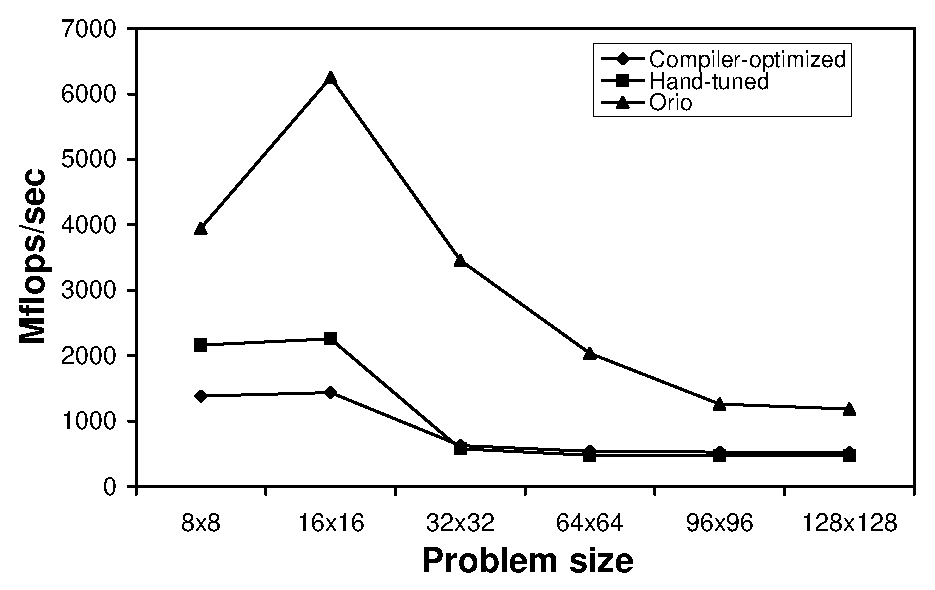
\includegraphics[width=.3\textwidth]{figures/ex27_cookie/smp.eps}
  \label{fig:ex27-cookie-smp} } \subfigure[Dual: $p=4$, $t/p=2$]{
  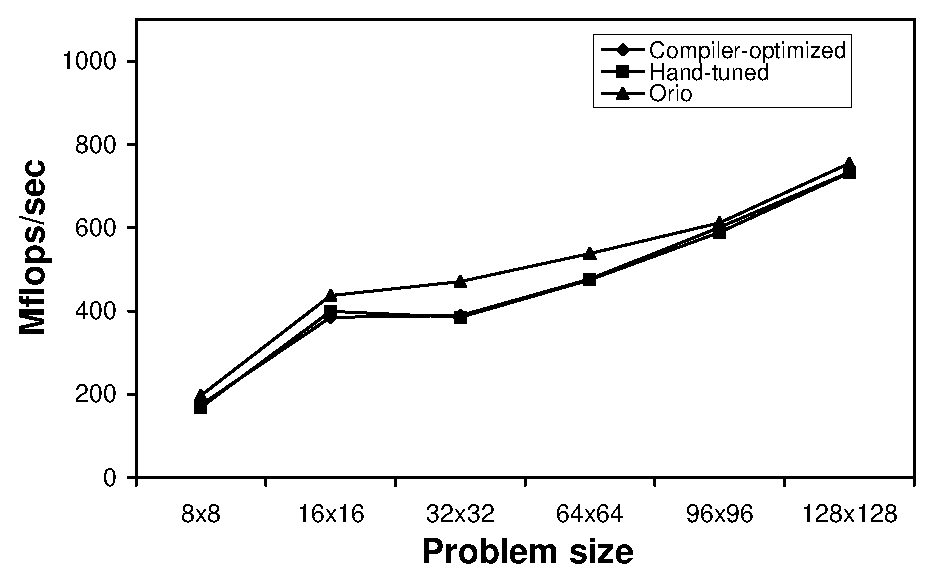
\includegraphics[width=.3\textwidth]{figures/ex27_cookie/dual.eps}
  \label{fig:ex27-cookie-dual} } \subfigure[VN: $p=8$, $t/p=1$]{
  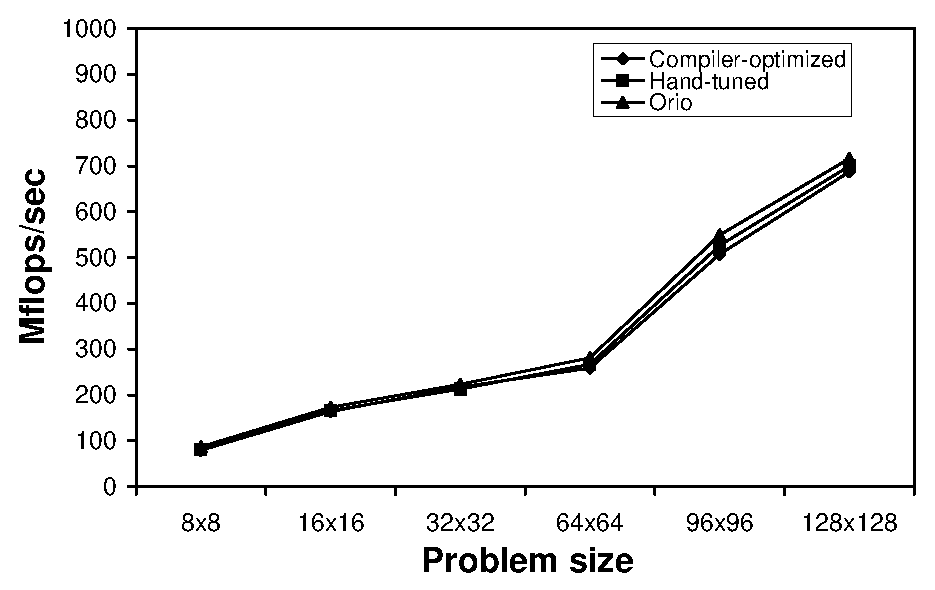
\includegraphics[width=.3\textwidth]{figures/ex27_cookie/vn.eps}
  \label{fig:ex27-cookie-vn} }
\end{center}
\vspace{-.2in} 
\caption{Performance of Inode SpMV on eight-core Intel machine; $p$ is the number of processes, $t/p$ is the threads per process.} 
\label{fig:ex27-cookie-results} 
\end{figure} 

\subsection{Irregular Computation Kernels} 

This section discusses the performance evaluations of the integrated
Pluto-Orio system (explained earlier in Section~\ref{sec:integration})
on the multicore Intel machine by using a number of application
kernels that are non-trivial to optimize and parallelize. We compare
the performance of the code tuned by Orio with the base code and the
Pluto-generated codes. The Pluto code was obtained via running the
base code with Pluto-0.3.0~\cite{pluto030} using \texttt{--tile} to
employ loop tiling for L1 cache,
\texttt{--l2tile} to employ loop tiling for L2 cache, and
\texttt{--unroll} to employ loop unrolling. Generating a parallel
version of Pluto code needs an additional \texttt{--parallel}
option. Note that we used Pluto's default tile sizes and unroll
factors to produce all Pluto codes. By default, Pluto always sets the
L1 tile sizes to 32x32 (or 32x32x32) and L2 tile sizes to 256x256 (or
256x256x256) depending on the loop nest depth. The default unroll
factors are always 64 for 1-D unrolling and 8x8 for 2-D
unroll/jamming. Furthermore, all codes were compiled with Intel C
Compiler using \texttt{-O3} optimization flag to ensure
auto-vectorization and other ICC optimizations, and \texttt{-parallel}
(or \texttt{-openmp}, when manual parallelization using OpenMP was
used) to enable code parallelization.
 
In the following sections, we refer to the ICC-optimized base code as
'Compiler-optimized', the Pluto-generated code with L1 tiling and
unroll/jamming as 'Pluto (L1 tiling)', and the Pluto-generated code
with L1 and L2 tilings and unroll/jamming as 'Pluto (L1+L2
tiling)'. Also, the code tuned by Orio is referred to as 'Pluto+Orio'.
 
\subsubsection{2-D Finite-Difference Time-Domain Method for Computational Electromagnetics}  
We consider the two-dimensional Finite Difference Time Domain (FDTD),
a popular method for solving computational electrodynamic problems. As
illustrated in Figure~\ref{fig:fdtd-2d-code}, the code of 
%
\begin{wrapfigure}{r}{3in}
\vspace{-0.2in}
\begin{center}
\begin{minipage}{3in} 
\scriptsize
\begin{verbatim} 
for(t=0; t<tmax; t++) { 
  for (j=0; j<ny; j++) 
    ey[0][j] = t; 
  for (i=1; i<nx; i++) 
    for (j=0; j<ny; j++) 
      ey[i][j] -= 0.5*(hz[i][j] - hz[i-1][j]); 
  for (i=0; i<nx; i++) 
    for (j=1; j<ny; j++) 
      ex[i][j] -= 0.5*(hz[i][j] - hz[i][j-1]); 
  for (i=0; i<nx; i++) 
    for (j=0; j<ny; j++) 
      hz[i][j] -= 0.7*(ex[i][j+1] - ex[i][j]
                  + ey[i+1][j] - ey[i][j]); 
} 
\end{verbatim} 
\end{minipage} 
\end{center}
\vspace{-0.2in}
\caption{2-D FDTD code} 
\label{fig:fdtd-2d-code} 
\end{wrapfigure}
%
2-D FDTD consists of four statements that are imperfectly nested. The arrays
$ex$ and $ey$ denote the electric fields, while the array $hz$ denotes
the magnetic field.

The performance of sequential 2-D FDTD codes for $tmax=500$ and
$nx=ny$ is presented in Figure~\ref{fig:fdtd-2d-cookie-seq}. The base
code optimized by ICC performs better than Pluto for small problem
sizes since all input arrays fit in the L2 cache, thus tiling
performed by Pluto will only introduce more overhead. As the array
sizes become larger, the lack of data reuse impairs the base code's
performance, whereas the Pluto performance remains steady. Code tuning
using Orio generates two code variants: one for small problem sizes
and another for large problem sizes. When the input array sizes are
small, Orio discovers that applying Pluto's polyhedral transformations
is not beneficial, and therefore, it employs only its syntactic
transformations on the original FDTD code. As to tuning for large
problem size, Orio exploits some of the Pluto's code transformations
and enhances it further with its syntactic optimizations, resulting in
performance constantly higher than both the base and Pluto codes. By
tuning the sequential code with Orio, the attainable performance
enhancement over Pluto is up to 86\%.
 
Figure~\ref{fig:fdtd-2d-cookie-par} displays the multicore performance
obtained for $tmax=500$ and $nx=ny=2000$. The results indicate that
while ICC is unable to auto-parallelize the code, Pluto detects the
existence of pipelined parallelism and then parallelizes the
code. Optimizing and tuning by Orio additionally improves the Pluto
performance by up to 78\%. Moreover, it can be seen that due to memory
contention between the two quad-core Intel processors, the performance
speedup of both the Pluto and Orio codes slightly decreases when the
number of used cores is greater than four.
 
\begin{figure}[htb] 
\begin{center} 
  \subfigure[Sequential (T=500)]{ 
  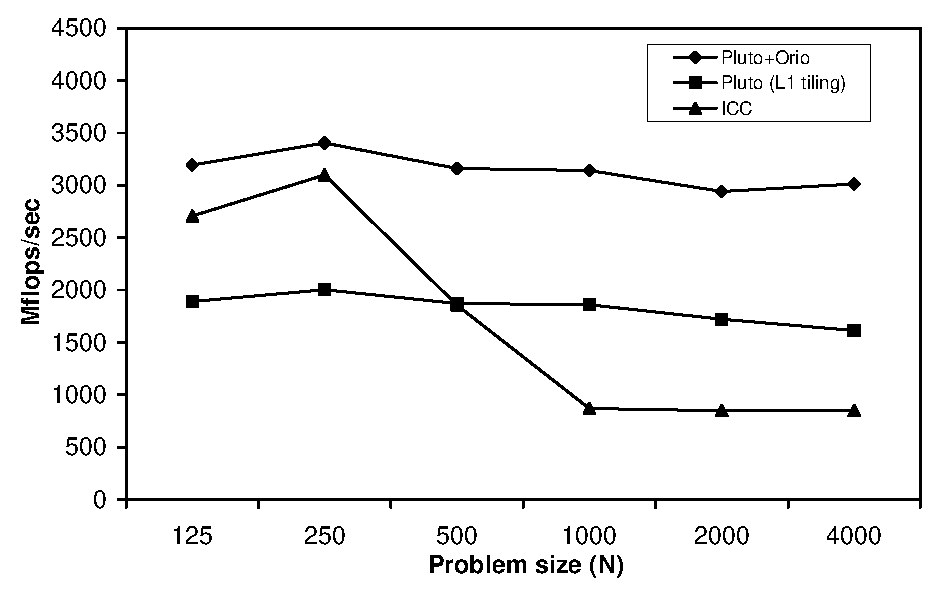
\includegraphics[width=.4\textwidth]{figures/fdtd-2d-cookie/seq.eps} 
  \label{fig:fdtd-2d-cookie-seq} } \subfigure[Parallel (T=500, 
  N=2000)]{ 
  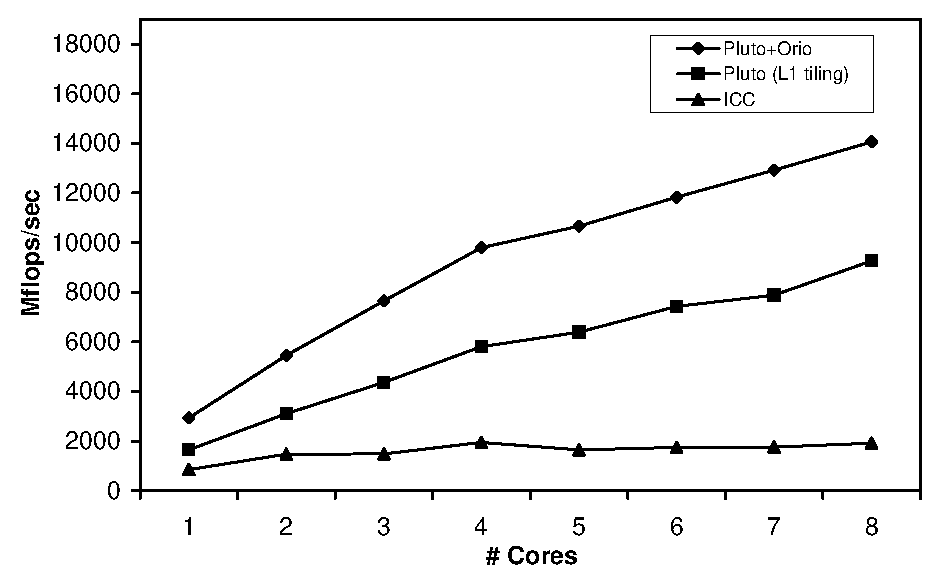
\includegraphics[width=.4\textwidth]{figures/fdtd-2d-cookie/par.eps} 
  \label{fig:fdtd-2d-cookie-par} } 
\end{center}
\vspace{-.2in} 
\caption{2-D FDTD performance on eight-core Intel machine} 
\label{fig:fdtd-2d-cookie-results} 
\vspace{-.2in}
\end{figure} 

%%BN: commented out since this needs more explanation (no room in this version)
%It is to be noted that collecting performance results of the Pluto 
%code with L1 and L2 tilings was not possible because of the large code 
%size of the generated loop nest, which led to an impractically huge 
%compile time. 
 
\subsubsection{3-D Gauss-Seidel Successive Over-Relaxation Method}  
Figure~\ref{fig:seidel-code} shows the 3-D Gauss-Seidel computation, 
which sometimes is referred to as
%
\begin{wrapfigure}{r}{3in}
\vspace{-0.2in}
\begin{center}
\begin{minipage}{3in} 
\scriptsize
\begin{verbatim} 
for (t=0; t<=T-1; t++) 
  for (i=1; i<=N-2; i++) 
    for (j=1; j<=N-2; j++) 
      A[i][j] = (A[i-1][j-1] + A[i-1][j] 
                + A[i-1][j+1] + A[i][j-1] 
                +A[i][j] + A[i][j+1] 
                + A[i+1][j-1] + A[i+1][j] 
                + A[i+1][j+1]) / 9.0; 
\end{verbatim} 
\end{minipage} 
\end{center}
\vspace{-0.1in}
\caption{3-D Gauss-Seidel code} 
\label{fig:seidel-code} 
\end{wrapfigure}
%
\emph{successive displacement method} to indicate the dependence of the iterations on the 
ordering. If the ordering is changed, the components of the new 
iterations will change as well. 
 
The sequential performance results shown in
Figure~\ref{fig:seidel-cookie-seq} are when $T=500$. As the figure
shows, applying Pluto's polyhedral tiling on the original code always
delivers performance boosts, which range from 126\% to
142\%. Performing two-level tiling (for both L1 and L2 caches) by
Pluto yields 13\% lower performance than only using L1 tiling; and
this is also reflected in the best sequential code found by Orio,
where one-level tiling (for L1 cache only) is always performed. The
sequential speedup obtained from tuning the Pluto code with Orio is
significant, ranging from 51\% to 133\%.

\begin{figure} [htb]
\begin{center} 
  \subfigure[Sequential (T=500)]{ 
  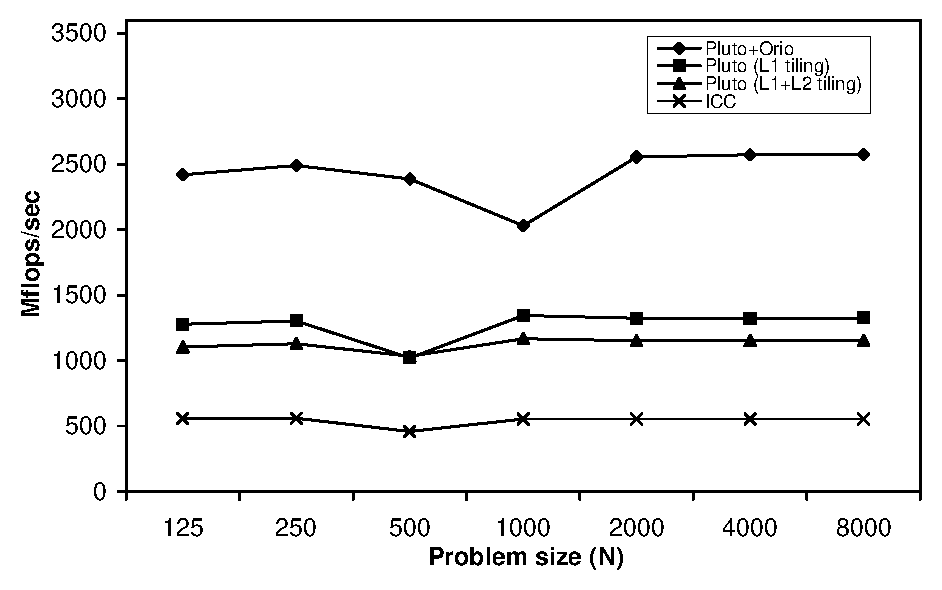
\includegraphics[width=.4\textwidth]{figures/seidel-cookie/seq.eps} 
  \label{fig:seidel-cookie-seq} } \subfigure[Parallel (T=500, 
  N=4000)]{ 
  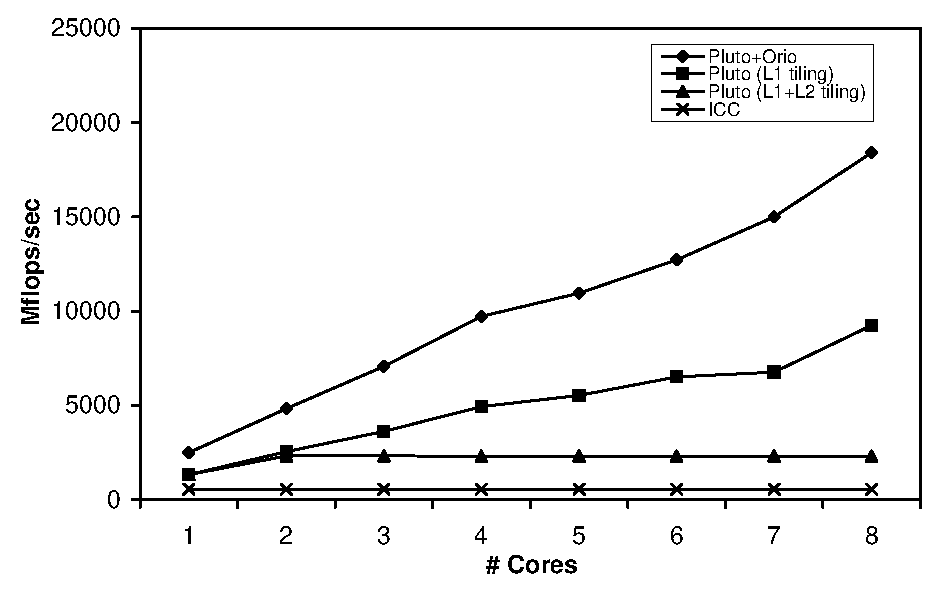
\includegraphics[width=.4\textwidth]{figures/seidel-cookie/par.eps} 
  \label{fig:seidel-cookie-par} } 
\end{center}
\vspace{-.2in} 
\caption{3-D Gauss-Seidel performance on eight-core Intel machine} 
\label{fig:seidel-cookie-results} 
\end{figure} 

Parallel performance for $T=500$ and $N=4000$ can be viewed in
Figure~\ref{fig:seidel-cookie-par}. Similar earlier trend also exists
in these performance results: Pluto parallelizes the code through its
polyhedral transformations (i.e., skewing and tiling), while the ICC
compiler alone does not parallelize the loop. Empirical tuning via
Orio creates up to 122\% speedups over the one-level tiled Pluto code,
and up to 548\% speedups over the two-level tiled Pluto code. Another
finding is that tiling for both L1 and L2 caches contributes to a poor
scalability because the number of tiles can be less than the number of
processors, resulting in underutilization of the available resources.

\subsubsection{LU Decomposition}  
 
LU Decomposition is a popular numerical method to solve linear
equation systems, and the 
%
\begin{wrapfigure}{r}{3in}
\begin{center}
\vspace{-.25in}
\begin{minipage}{2.8in} 
\scriptsize
\begin{verbatim} 
for (k=0; k<=N-1; k++) { 
  for (j=k+1; j<=N-1; j++) 
    A[k][j] /= A[k][k]; 
  for(i=k+1; i<=N-1; i++) 
    for (j=k+1; j<=N-1; j++) 
      A[i][j] -= A[i][k]*A[k][j]; 
} 
\end{verbatim} 
\end{minipage} 
\end{center}
\vspace{-0.2in}
\caption{LU Decomposition code} 
\label{fig:lu-code} 
\end{wrapfigure}
%
corresponding code is available in Figure~\ref{fig:lu-code}. 

The sequential performance results of LU Decomposition are presented
in Figure~\ref{fig:lu-cookie-seq}. Like 2-D FDTD, the ICC-optimized
code is more efficient than the Pluto-generated codes when the input
arrays are small and fit in the L2 cache. However, due to better data
locality, the performance of the Pluto-tiled codes exceeds the base
code as the input arrays get larger. Again, there are two different
codes generated by Orio: one for small problem sizes and one for large
problem sizes. And only the code tuned for large input arrays employs
Pluto's polyhedral transformations, prior to applying Orio's syntactic
transformations. Unlike 3-D Gauss-Seidel, this time Orio chooses to
apply both L1 and L2 tilings when generating the best tuned
code. Compared to the two Pluto codes, the Orio-tuned code yields
performance speedups in the range of 26\% to 277\%.

Parallel performance results shown in Figure~\ref{fig:lu-cookie-par}
were obtained for $N=4000$. From the results, we observe that ICC is
not able to parallelize the code, whereas Pluto achieves higher
performance by exploitation of multicore parallelism. Furthermore,
both Pluto-generated codes have comparable performance numbers, with a
slightly better scalability on the one-level tiled code. By the use of
Orio tuning, the performances of the Pluto base codes were improved by
a factor of 51\% to 120\%.
 
\begin{figure}[htb]
\begin{center} 
  \subfigure[Sequential]{ 
  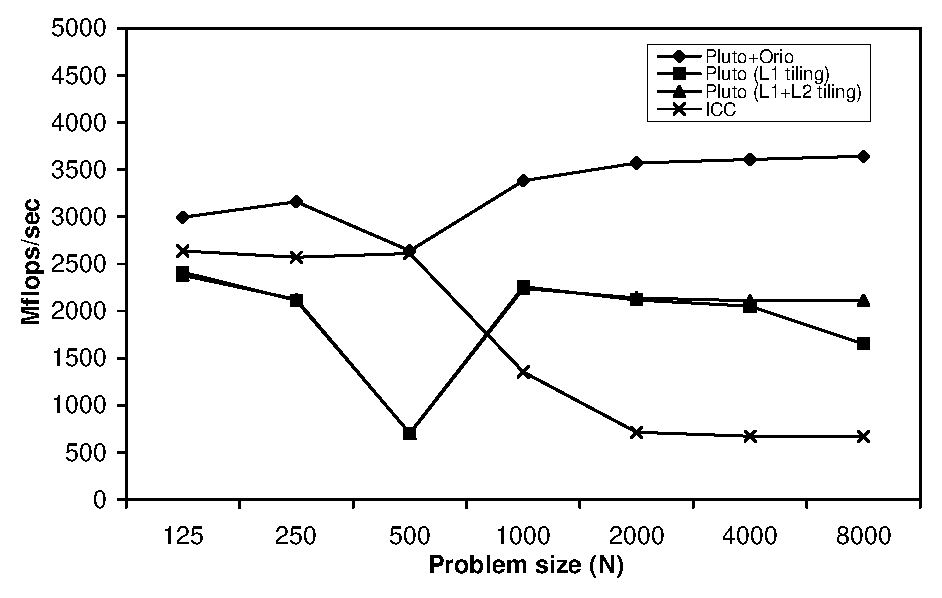
\includegraphics[width=.4\textwidth]{figures/lu-cookie/seq.eps} 
  \label{fig:lu-cookie-seq} } \subfigure[Parallel (N=4000)]{ 
  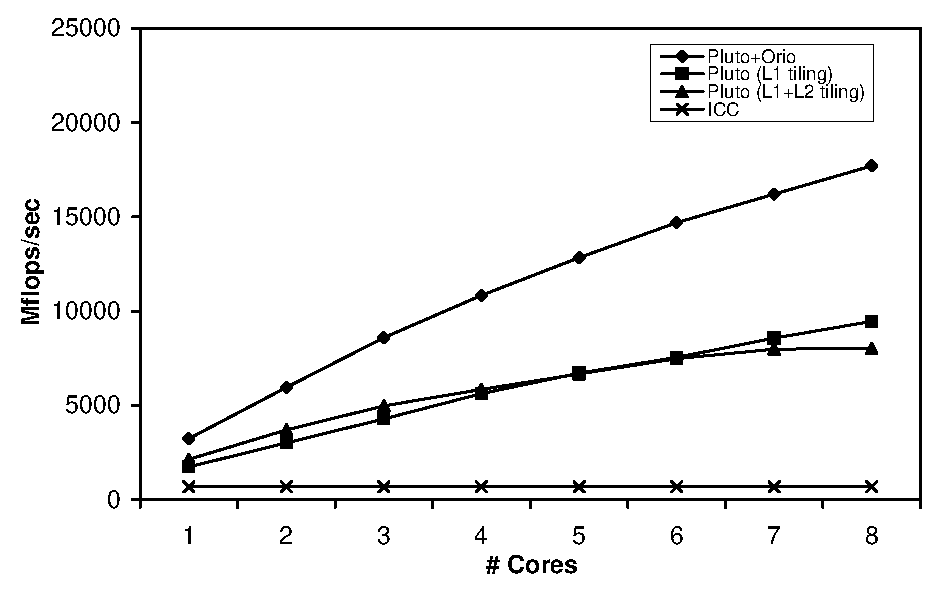
\includegraphics[width=.4\textwidth]{figures/lu-cookie/par.eps} 
  \label{fig:lu-cookie-par} } 
\end{center} 
\vspace{-.2in}
\caption{LU Decomposition performance on eight-core Intel machine} 
\label{fig:lu-cookie-results} 
\end{figure} 
 


